\documentclass[border=2mm]{standalone}
\usepackage{tikz}
\usetikzlibrary{calc}

\begin{document}

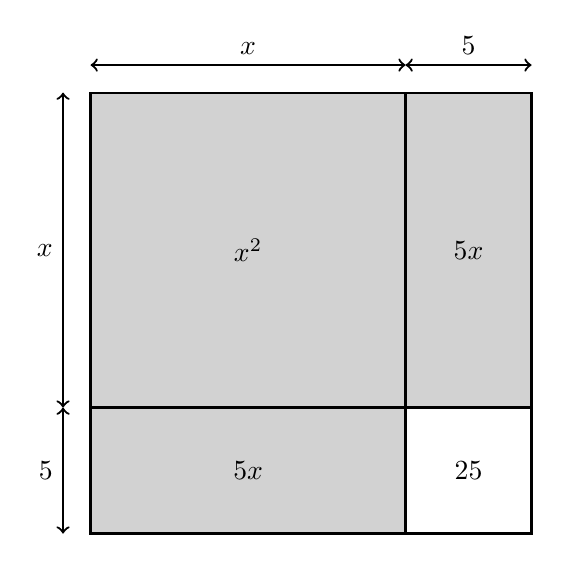
\begin{tikzpicture}
  \def\xside{4}
  \def\fivew{1.6}
  \def\pad{0.35}

  % nền
  \fill[gray!35] (0,\fivew) rectangle (\xside,\xside+\fivew);
  \fill[gray!35] (\xside,\fivew) rectangle (\xside+\fivew,\xside+\fivew);
  \fill[gray!35] (0,0) rectangle (\xside,\fivew);
  \fill[white]   (\xside,0) rectangle (\xside+\fivew,\fivew);

  % khung + chia
  \draw[thick] (0,0) rectangle (\xside+\fivew,\xside+\fivew);
  \draw[thick] (\xside,0) -- (\xside,\xside+\fivew);
  \draw[thick] (0,\fivew) -- (\xside+\fivew,\fivew);

  % nhãn (dùng calc để lấy trung điểm)
  \node at ($ (0,\fivew)!0.5!(\xside,\xside+\fivew) $) {$x^2$};
  \node at ($ (\xside,\fivew)!0.5!(\xside+\fivew,\xside+\fivew) $) {$5x$};
  \node at ($ (0,0)!0.5!(\xside,\fivew) $) {$5x$};
  \node at ($ (\xside,0)!0.5!(\xside+\fivew,\fivew) $) {$25$};

  % mũi tên trên
  \draw[<->,thick] (0,\xside+\fivew+\pad) -- node[above] {$x$}
                   (\xside,\xside+\fivew+\pad);
  \draw[<->,thick] (\xside,\xside+\fivew+\pad) -- node[above] {$5$}
                   (\xside+\fivew,\xside+\fivew+\pad);

  % mũi tên trái
  \draw[<->,thick] (-\pad,\fivew) -- node[left] {$x$}
                   (-\pad,\xside+\fivew);
  \draw[<->,thick] (-\pad,0) -- node[left] {$5$}
                   (-\pad,\fivew);
\end{tikzpicture}

\end{document}